\chapter{Trending}\label{trend}

We look at trends on Twitter and in finance and try to see if there are any
correlations between them. While defining the context of our research we made
some assumptions.

The Oslo stock exchange, OSEBX, is largely an oil based exchange, and
therefore we assume that oil related data will give a good indication of the
behavior of OSEBX. Section \ref{data:trend_data} says something about why we
choose tweets related to oil for the trend aggregation.

Further we wanted to look at trading that is not algorithm based. Algorithm
trading is also known as speed trading. So we started looking at technical
analysis. The technical analysis gives a base for decision support to the
trader. The techniques of technical analysis gives us good indications about
trends, but we want to take it further by involving sentiment analysis. 

We start by describing and defining a trend in section
\ref{trend:trend_is_your_friend}. 
Followed by trends in finance, \ref{trend:trends_in_finance}. 
Continuing with trends in relation to twitter, \ref{trend:trends_on_twitter}. 
And last we compare trends based on Twitter with finance trends, \ref{trend:compared}.
%

\section{The trend is your friend}\label{trend:trend_is_your_friend}
A trend is a series of changes that moves in the same direction over a period
of time. It is often associated with fashion or stock trading. The
definition of trend is "the general course or prevailing
tendency"\footnote{Dictionary.com:
\url{http://dictionary.referencs.com/browse/trend}}.

In finance the trend can be the deciding factor in buying or selling. Traders want
to buy during a bullish trend, while the value is going up. And they 
want to sell before you get to the bearish trend, when the value goes down.
Figure \ref{fig:stocktrends}, on page \pageref{fig:stocktrends}, shows basic
trends. When markets do not trend they move
sideways in trading ranges\footnote{Swing-trade-stocks.com:
\url{http://www.swing-trade-stocks.com/stock-trends.html}}.   

\begin{figure}[htb]
    \centering
    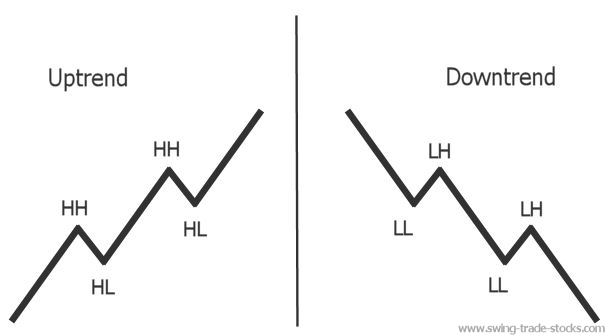
\includegraphics[width=\textwidth]{stocktrends.jpg} 
    \label{fig:stocktrends}
    \caption{Basic Trend}
Showing Higher Highs(HH), Lower Highs(LH), Higher Lows(HL), and Lower Lows(LL). 
\end{figure}

\textit{Moving average} and \textit{average directional index} are two
techniques in technical analysis. Moving averages, MA, can help to confirm a
move or determine a trend. Moving averages indicates average change over a
period of time. The time frame is often adjusted to the time the trader likes to
hold stocks before trading. Average directional index indicator, ADX, gives
clear, easy-to-read picture of the market, shown in figure
\ref{fig:adx_example_stock_trading}, on page
\pageref{fig:adx_example_stock_trading}. It shows if the trend strengthens or
weakens. We focus on the two described techniques later in this chapter.

When using ADX or other trend indicators it is difficult to spot or predict the
trend. When trading is based on a trend, the problem is to find
the trend and prolong it into the future. This is where we combine Twitter
with traditional trading. If we could predict the trend based on public opinion
mined from Twitter, we would have an advantage over the traditional trader. 

Data is increasingly important for trend prediction. The better data we have,
the more accurate the trend we predict can be. By focusing on sentiment we aim
for the cooperation of information available on the Internet and the value of
sentiment to predict trends. This will be more important in the future. 

If the trend is your friend, you know how the market will move and make
good decisions in accordance with it. 
%

\section{Trending in Finance}\label{trend:trends_in_finance}
Moving average(MA), and average directional index(ADX) are the two trend
indication techniques we test in this thesis. 

\paragraph{Moving Average(MA)}
\hspace{0pt}\\
\begin{figure}[htb]
    \centering
    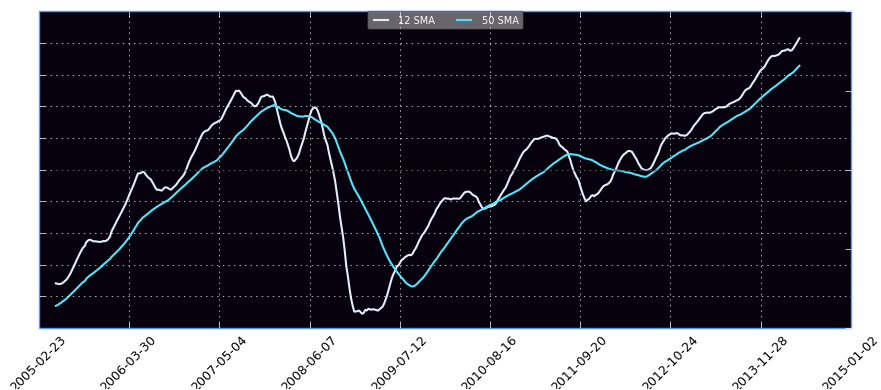
\includegraphics[width=\textwidth]{moving_average_example.png}
    \label{fig:moving_average_example}
    \caption{Moving Average example}
The figure show the Moving Average for OSEBX from march 2005 until May 2014. The
blue MA has a time frame of 50 weeks, while the white MA has a time frame of 12
weeks. 
\end{figure}

MA\footnote{Wikipedia: \url{https://en.wikipedia.org/wiki/Moving_average}} is
the unweighted mean of the previous n days. Given the closing price of the last
n days as: 

\math{
p_M, p_{M-1},\dots,p_{M-(n-1)}
}\\

We have that the simple moving average is: 

\math{
\textit{SMA} = { p_M + p_{M-1} + \cdots + p_{M-(n-1)} \over n }
}\\

There are also other variants of the moving average. Such as cumulative MA,
weighted MA and exponential MA. We use the simple version for MA trend. 

\paragraph{Average Directional Index (ADX)}
\hspace{0pt}\\

\begin{figure}[htb]
    \centering
    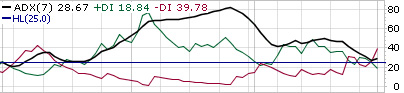
\includegraphics[width=\textwidth]{adx_example_stock_trading.jpg}
    \label{fig:adx_example_stock_trading}
    \caption{Average Directional Index example}
An example of ADX. Green line is showing increase in price. Red line is
decrease in price. The black line is the ADX.
\end{figure}
In ADX, the further away from each other the red and green lines are, the
stronger the trend is. 

ADX\footnote{Wikipedia:
\url{https://en.wikipedia.org/wiki/Average_Directional_Index}} uses the positive directional indicator(+DI) and the negative directional
indicator(-DI) in combination to determine a trend. The high, low and closing
values are needed for the ADX to be calculated. The directional movement is
calculated as follows: 
\begin{verbatim}
UpMove = today's high - yesterday's high
DownMove = yesterday's low - today's low
if UpMove > DownMove and UpMove > 0, then +DM = UpMove, else +DM = 0
if DownMove > UpMove and DownMove > 0, then -DM = DownMove, else -DM = 0 
\end{verbatim} 

When the directions are calculated we choose the time frame we want to
investigate. And get -DI and +DI as follows:\footnote{Wikipedia:
\url{https://en.wikipedia.org/wiki/Average_True_Range}}
\begin{verbatim}
+DI = 100 times exponential moving average of +DM 
      divided by average true range
-DI = 100 times exponential moving average of -DM 
      divided by average true range 
\end{verbatim} 

Where the time frame defines the number of periods used in the exponential
moving average. And the average true is an exponential average of the true
range. Resulting in the ADX:
\begin{verbatim}
ADX = 100 times the exponential moving average 
      of the absolute value of (+DI - -DI) 
      divided by (+DI + -DI)
\end{verbatim}
%

\paragraph{Experiments}
\hspace{0pt}\\
In the experiment, section \ref{experiments:trend} on page
\pageref{experiments:trend}, we plot the graph for
the finance trends. In the experiment we used data from OSEBX. The same time
frame was used for stock data and tweet data, Apr 26 - May 26.
%

\section{Twitter based Trends}\label{trend:trends_on_twitter}
We have two trends with twitter. First the trends Twitter themselves
create based on words or hashtags that appear in many tweets. Second the trend we
compile ourselves based on the trend data described in section
\ref{data:trend_data}, page \pageref{data:trend_data}. 

\paragraph{Trends on Twitter}
\hspace{0pt}\\
On Twitter.com there is a feature called 'Trends'. It shows the words that are
used the most recently. A screen capture of it can be seen in figure
\ref{fig:trends_on_twitter}, page \pageref{fig:trends_on_twitter}.

\begin{figure}[htb]
	\centering
    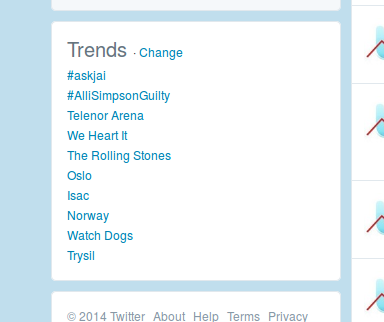
\includegraphics[width=0.5\textwidth]{trends_on_twitter.png}
    \label{fig:trends_on_twitter}
    \caption{Trends on Twitter}
Screen capture of trends from Twitter.
\end{figure}

The trends on Twitter are in many cases predictable and adds little value to trend
compilation. The trend on Twitter is also specialised for each user, based on
that users subscriptions and location. As an example at the Norwegian national
day(May 17.) we would have trending words like \textit{Norge}, \textit{Norway},
and \textit{\#17Mai}. Today we already know that this will happen again next
year.
%

\paragraph{Twitter based sentiment trend} 
\hspace{0pt}\\
% what & why.
With the trend calculations based on sentiment we looked at methods used in
finance and took inspiration from that. We ended up choosing the two
previously mentioned methods MA and ADX as a base for our own work. 

By using the two existing methods a base for our aggregated trend we gain a
good indication of weather or not this is a viable way of creating trends with sentiment data.

The new element we use with the MA and ADX methods is the sentiment analysis.
By using sentiment data we hope to create a sentiment trend. As far as we have
research no one else has done this before. 

As we do new and untested things we have no guarantee of success. But we have a
good opportunity to test uses for sentiment analysis. 

The trick to our method lies in the data manipulation. We manipulate the
sentiment data we have to fit the existing format of stock data. Then we run
the MA and ADX methods with the sentiment data to see if it works.  

What we do, results in two methods of trend aggregation. Sentiment based MA and
sentiment based ADX. 
 
% how
Using the trend data described in section \ref{data:trend_data} we construct
the MA and ADX graphs based on sentiment. The data consists of tweets and is
based on Twitter handles for users with big impact in the oil industry. There
are two parts to the data. First tweets from Norwegian users, and secondly
tweets from international users. To simplify the trend creation a bit we used
English tweets, ignoring tweets in Norwegian. After sorting the mined tweets by
day, we classify all tweets for each day. The classification from each day is
referred to as a trend day. The trend day contains the amount of positive
tweets, the amount of negative tweets, and the total amount of tweets collected
for that day. 

\begin{python}
trend_days = {
	'trend-Apr-30': {'neg': 112, 'pos': 131, 'tot': 243},
    'trend-May-19': {'neg': 523, 'pos': 1326, 'tot': 1849},
    'trend-May-18': {'neg': 59, 'pos': 110, 'tot': 169},
    'trend-May-15': {'neg': 1151, 'pos': 2255, 'tot': 3406},
}
\end{python}  

Now we have some sentiment data to create a trend from. To simplify the trend
aggregation and the graph plotting, we transform the data to fit into the
format used for the finance data. The format of the data is the well known
'comma separated values', CSV.  

\begin{verbatim}
Date,close,high,low,open,volume
20140423,559.41,562.45,557.74,561.13,0
20140424,562.89,565.65,559.84,559.41,0
20140425,566.24,566.24,562.41,562.89,0
20140428,566.82,567.14,564.55,566.24,0
\end{verbatim}

To transform the data we do the following: 
\begin{python}
trend_days = get_tweet_trend_data()
keys = sorted(trend_days.keys())
date = ""
for i in range(1, len(keys)):
    if "Apr" in keys[i]:
        date = "201404" + str(keys[i].split('-')[2])
    elif "May" in keys[i]:
        date = "201405" + str(keys[i].split('-')[2])
    volume = trend_days[keys[i]]['tot'] * 1.0
    # (positive_tweets / total_amount_of_tweets)*scale
    high = (trend_days[keys[i]]['pos'] / volume) * 1000
    # (negative_teets / total_amount_of_tweets)*scale
    low = (trend_days[keys[i]]['neg'] / volume) * 1000
    openv = 0
    close = high - low
    print str(date) + "," + str(close) + "," + str(high) \
          + str(",") +str(low) + "," + str(volume / 10) + \
          "," + str(0)
\end{python}

We scale the values to plot a more representative graph. All the
proportions are kept intact, so the MA and ADX are still valid.
This method is tested in section \ref{experiments:trend} on page
\pageref{experiments:trend}.
% 

\section{Comparing the Trends}\label{trend:compared}
Comparing the finance trend and the Twitter based trend is easy. We compare the
two graphs, look for similarities, and draw conclusions. Drawing conclusions is
the difficult part.

For plot examples see figure \ref{fig:trend_finance_plot}, page
\pageref{fig:trend_finance_plot}, and figure \ref{fig:trend_tweet_plot}, page
\pageref{fig:trend_tweet_plot}.

We look at the two plotted trends, the MA and the ADX. More specifically we
compare the white MA of both graphs with each other, and the blue MA lines of
each graph with each other. And look for similarities. With the ADX we will look
for similar movements and turning points in the graphs. Also areas where the
red and green lines stay apart.  

Comparison should give some conclusions of the trustworthiness of the
sentiment trend. For traders to trust in the sentiment analysis as a new way of
predicting trends the sentiment would have to provide profit and scientifically
proven results. At this stage there would be few who would rely on sentiment
analysis as a trend indicator of the stock market. The trust lies in the
technical analysis.  

With the comparison we have the drawback of examining a stock exchange instead
of a single stock. Comparing one stock at a time would give better indications of
the accuracy of the sentiment trend. This should be explored further in the
future.   
%

\section{Future work}
For future improvements of the trend aggregation we should explore three aspects.
One, the Norwegian market we started with. Two, the oil tweets. Three, find
out whether or not oil tweets are a good indication of the OSEBX. 

Additionally we should look into single stocks in the comparison of indicators.
This way we can explore 'stock vs stock' Twitter trends, and find new information
there.
%
